
%% bare_conf.tex
%% V1.3
%% 2007/01/11
%% by Michael Shell
%% See:
%% http://www.michaelshell.org/
%% for current contact information.
%%
%% This is a skeleton file demonstrating the use of IEEEtran.cls
%% (requires IEEEtran.cls version 1.7 or later) with an IEEE conference paper.
%%
%% Support sites:
%% http://www.michaelshell.org/tex/ieeetran/
%% http://www.ctan.org/tex-archive/macros/latex/contrib/IEEEtran/
%% and
%% http://www.ieee.org/

%%*************************************************************************
%% Legal Notice:
%% This code is offered as-is without any warranty either expressed or
%% implied; without even the implied warranty of MERCHANTABILITY or
%% FITNESS FOR A PARTICULAR PURPOSE! 
%% User assumes all risk.
%% In no event shall IEEE or any contributor to this code be liable for
%% any damages or losses, including, but not limited to, incidental,
%% consequential, or any other damages, resulting from the use or misuse
%% of any information contained here.
%%
%% All comments are the opinions of their respective authors and are not
%% necessarily endorsed by the IEEE.
%%
%% This work is distributed under the LaTeX Project Public License (LPPL)
%% ( http://www.latex-project.org/ ) version 1.3, and may be freely used,
%% distributed and modified. A copy of the LPPL, version 1.3, is included
%% in the base LaTeX documentation of all distributions of LaTeX released
%% 2003/12/01 or later.
%% Retain all contribution notices and credits.
%% ** Modified files should be clearly indicated as such, including  **
%% ** renaming them and changing author support contact information. **
%%
%% File list of work: IEEEtran.cls, IEEEtran_HOWTO.pdf, bare_adv.tex,
%%                    bare_conf.tex, bare_jrnl.tex, bare_jrnl_compsoc.tex
%%*************************************************************************

% *** Authors should verify (and, if needed, correct) their LaTeX system  ***
% *** with the testflow diagnostic prior to trusting their LaTeX platform ***
% *** with production work. IEEE's font choices can trigger bugs that do  ***
% *** not appear when using other class files.                            ***
% The testflow support page is at:
% http://www.michaelshell.org/tex/testflow/



% Note that the a4paper option is mainly intended so that authors in
% countries using A4 can easily print to A4 and see how their papers will
% look in print - the typesetting of the document will not typically be
% affected with changes in paper size (but the bottom and side margins will).
% Use the testflow package mentioned above to verify correct handling of
% both paper sizes by the user's LaTeX system.
%
% Also note that the "draftcls" or "draftclsnofoot", not "draft", option
% should be used if it is desired that the figures are to be displayed in
% draft mode.
%
\documentclass[conference]{IEEEtran}
% Add the compsoc option for Computer Society conferences.
%
% If IEEEtran.cls has not been installed into the LaTeX system files,
% manually specify the path to it like:
% \documentclass[conference]{../sty/IEEEtran}


\usepackage{pgfplots}
\usepackage{algorithm}
\usepackage{amsmath}
\usepackage{mathtools}
\usepackage{graphicx}

% Some very useful LaTeX packages include:
% (uncomment the ones you want to load)


% *** MISC UTILITY PACKAGES ***
%
%\usepackage{ifpdf}
% Heiko Oberdiek's ifpdf.sty is very useful if you need conditional
% compilation based on whether the output is pdf or dvi.
% usage:
% \ifpdf
%   % pdf code
% \else
%   % dvi code
% \fi
% The latest version of ifpdf.sty can be obtained from:
% http://www.ctan.org/tex-archive/macros/latex/contrib/oberdiek/
% Also, note that IEEEtran.cls V1.7 and later provides a builtin
% \ifCLASSINFOpdf conditional that works the same way.
% When switching from latex to pdflatex and vice-versa, the compiler may
% have to be run twice to clear warning/error messages.






% *** CITATION PACKAGES ***
%
\usepackage{cite}
% cite.sty was written by Donald Arseneau
% V1.6 and later of IEEEtran pre-defines the format of the cite.sty package
% \cite{} output to follow that of IEEE. Loading the cite package will
% result in citation numbers being automatically sorted and properly
% "compressed/ranged". e.g., [1], [9], [2], [7], [5], [6] without using
% cite.sty will become [1], [2], [5]--[7], [9] using cite.sty. cite.sty's
% \cite will automatically add leading space, if needed. Use cite.sty's
% noadjust option (cite.sty V3.8 and later) if you want to turn this off.
% cite.sty is already installed on most LaTeX systems. Be sure and use
% version 4.0 (2003-05-27) and later if using hyperref.sty. cite.sty does
% not currently provide for hyperlinked citations.
% The latest version can be obtained at:
% http://www.ctan.org/tex-archive/macros/latex/contrib/cite/
% The documentation is contained in the cite.sty file itself.






% *** GRAPHICS RELATED PACKAGES ***
%
\ifCLASSINFOpdf
  % \usepackage[pdftex]{graphicx}
  % declare the path(s) where your graphic files are
  % \graphicspath{{../pdf/}{../jpeg/}}
  % and their extensions so you won't have to specify these with
  % every instance of \includegraphics
  % \DeclareGraphicsExtensions{.pdf,.jpeg,.png}
\else
  % or other class option (dvipsone, dvipdf, if not using dvips). graphicx
  % will default to the driver specified in the system graphics.cfg if no
  % driver is specified.
  % \usepackage[dvips]{graphicx}
  % declare the path(s) where your graphic files are
  % \graphicspath{{../eps/}}
  % and their extensions so you won't have to specify these with
  % every instance of \includegraphics
  % \DeclareGraphicsExtensions{.eps}
\fi
% graphicx was written by David Carlisle and Sebastian Rahtz. It is
% required if you want graphics, photos, etc. graphicx.sty is already
% installed on most LaTeX systems. The latest version and documentation can
% be obtained at: 
% http://www.ctan.org/tex-archive/macros/latex/required/graphics/
% Another good source of documentation is "Using Imported Graphics in
% LaTeX2e" by Keith Reckdahl which can be found as epslatex.ps or
% epslatex.pdf at: http://www.ctan.org/tex-archive/info/
%
% latex, and pdflatex in dvi mode, support graphics in encapsulated
% postscript (.eps) format. pdflatex in pdf mode supports graphics
% in .pdf, .jpeg, .png and .mps (metapost) formats. Users should ensure
% that all non-photo figures use a vector format (.eps, .pdf, .mps) and
% not a bitmapped formats (.jpeg, .png). IEEE frowns on bitmapped formats
% which can result in "jaggedy"/blurry rendering of lines and letters as
% well as large increases in file sizes.
%
% You can find documentation about the pdfTeX application at:
% http://www.tug.org/applications/pdftex





% *** MATH PACKAGES ***
%
%\usepackage[cmex10]{amsmath}
% A popular package from the American Mathematical Society that provides
% many useful and powerful commands for dealing with mathematics. If using
% it, be sure to load this package with the cmex10 option to ensure that
% only type 1 fonts will utilized at all point sizes. Without this option,
% it is possible that some math symbols, particularly those within
% footnotes, will be rendered in bitmap form which will result in a
% document that can not be IEEE Xplore compliant!
%
% Also, note that the amsmath package sets \interdisplaylinepenalty to 10000
% thus preventing page breaks from occurring within multiline equations. Use:
%\interdisplaylinepenalty=2500
% after loading amsmath to restore such page breaks as IEEEtran.cls normally
% does. amsmath.sty is already installed on most LaTeX systems. The latest
% version and documentation can be obtained at:
% http://www.ctan.org/tex-archive/macros/latex/required/amslatex/math/




% *** SPECIALIZED LIST PACKAGES ***
%
\usepackage{algorithmic}
% algorithmic.sty was written by Peter Williams and Rogerio Brito.
% This package provides an algorithmic environment fo describing algorithms.
% You can use the algorithmic environment in-text or within a figure
% environment to provide for a floating algorithm. Do NOT use the algorithm
% floating environment provided by algorithm.sty (by the same authors) or
% algorithm2e.sty (by Christophe Fiorio) as IEEE does not use dedicated
% algorithm float types and packages that provide these will not provide
% correct IEEE style captions. The latest version and documentation of
% algorithmic.sty can be obtained at:
% http://www.ctan.org/tex-archive/macros/latex/contrib/algorithms/
% There is also a support site at:
% http://algorithms.berlios.de/index.html
% Also of interest may be the (relatively newer and more customizable)
% algorithmicx.sty package by Szasz Janos:
% http://www.ctan.org/tex-archive/macros/latex/contrib/algorithmicx/




% *** ALIGNMENT PACKAGES ***
%
%\usepackage{array}
% Frank Mittelbach's and David Carlisle's array.sty patches and improves
% the standard LaTeX2e array and tabular environments to provide better
% appearance and additional user controls. As the default LaTeX2e table
% generation code is lacking to the point of almost being broken with
% respect to the quality of the end results, all users are strongly
% advised to use an enhanced (at the very least that provided by array.sty)
% set of table tools. array.sty is already installed on most systems. The
% latest version and documentation can be obtained at:
% http://www.ctan.org/tex-archive/macros/latex/required/tools/


%\usepackage{mdwmath}
%\usepackage{mdwtab}
% Also highly recommended is Mark Wooding's extremely powerful MDW tools,
% especially mdwmath.sty and mdwtab.sty which are used to format equations
% and tables, respectively. The MDWtools set is already installed on most
% LaTeX systems. The lastest version and documentation is available at:
% http://www.ctan.org/tex-archive/macros/latex/contrib/mdwtools/


% IEEEtran contains the IEEEeqnarray family of commands that can be used to
% generate multiline equations as well as matrices, tables, etc., of high
% quality.


%\usepackage{eqparbox}
% Also of notable interest is Scott Pakin's eqparbox package for creating
% (automatically sized) equal width boxes - aka "natural width parboxes".
% Available at:
% http://www.ctan.org/tex-archive/macros/latex/contrib/eqparbox/





% *** SUBFIGURE PACKAGES ***
%\usepackage[tight,footnotesize]{subfigure}
% subfigure.sty was written by Steven Douglas Cochran. This package makes it
% easy to put subfigures in your figures. e.g., "Figure 1a and 1b". For IEEE
% work, it is a good idea to load it with the tight package option to reduce
% the amount of white space around the subfigures. subfigure.sty is already
% installed on most LaTeX systems. The latest version and documentation can
% be obtained at:
% http://www.ctan.org/tex-archive/obsolete/macros/latex/contrib/subfigure/
% subfigure.sty has been superceeded by subfig.sty.



% \usepackage[caption=false]{caption}
% \usepackage[font=footnotesize]{subfig}
% subfig.sty, also written by Steven Douglas Cochran, is the modern
% replacement for subfigure.sty. However, subfig.sty requires and
% automatically loads Axel Sommerfeldt's caption.sty which will override
% IEEEtran.cls handling of captions and this will result in nonIEEE style
% figure/table captions. To prevent this problem, be sure and preload
% caption.sty with its "caption=false" package option. This is will preserve
% IEEEtran.cls handing of captions. Version 1.3 (2005/06/28) and later 
% (recommended due to many improvements over 1.2) of subfig.sty supports
% the caption=false option directly:
%\usepackage[caption=false,font=footnotesize]{subfig}
%
% The latest version and documentation can be obtained at:
% http://www.ctan.org/tex-archive/macros/latex/contrib/subfig/
% The latest version and documentation of caption.sty can be obtained at:
% http://www.ctan.org/tex-archive/macros/latex/contrib/caption/




% *** FLOAT PACKAGES ***
%
% \usepackage{fixltx2e}
% fixltx2e, the successor to the earlier fix2col.sty, was written by
% Frank Mittelbach and David Carlisle. This package corrects a few problems
% in the LaTeX2e kernel, the most notable of which is that in current
% LaTeX2e releases, the ordering of single and double column floats is not
% guaranteed to be preserved. Thus, an unpatched LaTeX2e can allow a
% single column figure to be placed prior to an earlier double column
% figure. The latest version and documentation can be found at:
% http://www.ctan.org/tex-archive/macros/latex/base/



\usepackage{stfloats}
% stfloats.sty was written by Sigitas Tolusis. This package gives LaTeX2e
% the ability to do double column floats at the bottom of the page as well
% as the top. (e.g., "\begin{figure*}[!b]" is not normally possible in
% LaTeX2e). It also provides a command:
%\fnbelowfloat
% to enable the placement of footnotes below bottom floats (the standard
% LaTeX2e kernel puts them above bottom floats). This is an invasive package
% which rewrites many portions of the LaTeX2e float routines. It may not work
% with other packages that modify the LaTeX2e float routines. The latest
% version and documentation can be obtained at:
% http://www.ctan.org/tex-archive/macros/latex/contrib/sttools/
% Documentation is contained in the stfloats.sty comments as well as in the
% presfull.pdf file. Do not use the stfloats baselinefloat ability as IEEE
% does not allow \baselineskip to stretch. Authors submitting work to the
% IEEE should note that IEEE rarely uses double column equations and
% that authors should try to avoid such use. Do not be tempted to use the
% cuted.sty or midfloat.sty packages (also by Sigitas Tolusis) as IEEE does
% not format its papers in such ways.





% *** PDF, URL AND HYPERLINK PACKAGES ***
%
%\usepackage{url}
% url.sty was written by Donald Arseneau. It provides better support for
% handling and breaking URLs. url.sty is already installed on most LaTeX
% systems. The latest version can be obtained at:
% http://www.ctan.org/tex-archive/macros/latex/contrib/misc/
% Read the url.sty source comments for usage information. Basically,
% \url{my_url_here}.

% *** Do not adjust lengths that control margins, column widths, etc. ***
% *** Do not use packages that alter fonts (such as pslatex).         ***
% There should be no need to do such things with IEEEtran.cls V1.6 and later.
% (Unless specifically asked to do so by the journal or conference you plan
% to submit to, of course. )


% correct bad hyphenation here
\hyphenation{op-tical net-works semi-conduc-tor}


\begin{document}
%
% paper title
% can use linebreaks \\ within to get better formatting as desired
\title{Modeling Metal Protein Complexes from Experimental Extended X-ray Absorption Fine Structure using Evolutionary Algorithms}


% author names and affiliations
% use a multiple column layout for up to three different
% affiliations
\author{
  \IEEEauthorblockN{Collin Price}
  \IEEEauthorblockA{Brock University\\
  St. Catharines, Ontario\\
  Email: cp06vz@brocku.ca}
  \and
  \IEEEauthorblockN{Sheridan Houghten}
  \IEEEauthorblockA{Brock University\\
  St. Catharines, Ontario\\
  Email: houghten@brocku.ca}
  \and
  \IEEEauthorblockN{Sergey Vassiliev}
  \IEEEauthorblockA{Brock University\\
  St. Catharines, Ontario\\
  Email: svassiliev@brocku.ca}
  \and
  \IEEEauthorblockN{Doug Bruce}
  \IEEEauthorblockA{Brock University\\
  St. Catharines, Ontario\\
  Email: dbruce@brocku.ca}
}
% conference papers do not typically use \thanks and this command
% is locked out in conference mode. If really needed, such as for
% the acknowledgment of grants, issue a \IEEEoverridecommandlockouts
% after \documentclass

% for over three affiliations, or if they all won't fit within the width
% of the page, use this alternative format:
% 
% \author{\IEEEauthorblockN{Michael Shell\IEEEauthorrefmark{1},
% Homer Simpson\IEEEauthorrefmark{2},
% James Kirk\IEEEauthorrefmark{3}, 
% Montgomery Scott\IEEEauthorrefmark{3} and
% Eldon Tyrell\IEEEauthorrefmark{4}}
% \IEEEauthorblockA{\IEEEauthorrefmark{1}School of Electrical and Computer Engineering\\
% Georgia Institute of Technology,
% Atlanta, Georgia 30332--0250\\ Email: see http://www.michaelshell.org/contact.html}
% \IEEEauthorblockA{\IEEEauthorrefmark{2}Twentieth Century Fox, Springfield, USA\\
% Email: homer@thesimpsons.com}
% \IEEEauthorblockA{\IEEEauthorrefmark{3}Starfleet Academy, San Francisco, California 96678-2391\\
% Telephone: (800) 555--1212, Fax: (888) 555--1212}
% \IEEEauthorblockA{\IEEEauthorrefmark{4}Tyrell Inc., 123 Replicant Street, Los Angeles, California 90210--4321}}




% use for special paper notices
%\IEEEspecialpapernotice{(Invited Paper)}




% make the title area
\maketitle


\begin{abstract}
%\boldmath

Experimental \textit{extended x-ray absorption fine structure} (EXAFS) spectra carry information about the chemical structure of metal protein complexes. However, predicting the structure of such complexes from EXAFS spectra is not a simple task. Currently methods such as Monte Carlo Optimization or simulated annealing are used in structure refinement of EXAFS. These methods have proved somewhat successful in structure refinement but have not been successful in finding the global minima. Based on the success of using evolutionary algorithms to overcome local minima issues in other domains, we propose multiple approaches to better predict the structure of metal protein complexes; genetic algorithm (GA), particle swarm optimization (PSO), and differential evolution (DE).

\end{abstract}
% IEEEtran.cls defaults to using nonbold math in the Abstract.
% This preserves the distinction between vectors and scalars. However,
% if the conference you are submitting to favors bold math in the abstract,
% then you can use LaTeX's standard command \boldmath at the very start
% of the abstract to achieve this. Many IEEE journals/conferences frown on
% math in the abstract anyway.

% no keywords
\begin{IEEEkeywords}
Molecular Structure, Evolutionary Algorithms, Representation, Recentering-Restarting, Particle Swarm Optimization, Extended X-ray Absorption Fine Structure,
\end{IEEEkeywords}



% For peer review papers, you can put extra information on the cover
% page as needed:
% \ifCLASSOPTIONpeerreview
% \begin{center} \bfseries EDICS Category: 3-BBND \end{center}
% \fi
%
% For peerreview papers, this IEEEtran command inserts a page break and
% creates the second title. It will be ignored for other modes.
\IEEEpeerreviewmaketitle

\section{Introduction}

The goal of this work is to explore different types of evolutionary algorithms in an effort to find the exact molecular structure of a molecule given experimental extended X-ray absorption fine structure (EXAFS) spectra. EXAFS experiments are an effective way of determining a molecule's molecular structure. EXAFS experiments are unique in that they can be used on a variety of materials, including gas and liquids. 

For the experiments a non-protein chemical compound found within proteins is used. The oxygen-evolving complex (OEC) is required to catalyze the oxidation of water to produce dioxygen. There is a high quality experimental EXAFS spectra of OEC in S$_1$-state that will be used to create a comparative measure against the results. The goal is to create a calculated molecular structure that closely resembles the experimental EXAFS spectra. Finding a good molecular structure for the OEC is important in understanding the catalytic cycle and the development of biomimetics~\cite{luber2011s1}.

Currently such methods as computational chemistry~\cite{hsiao2006exafs}, quantum mechanics~\cite{hsiao2006exafs}~\cite{sproviero2008model}, and conjugate gradient optimization~\cite{luber2011s1} are being used to determine the molecular structure of compounds. The problem with these approaches is that they are converging on local minima. A major difficulty with molecular structure refinement is that there are too many degrees of freedom involved. With respect to the OEC there are 79 degrees of freedom, corresponding to the 79 atoms in the OEC. See Figure~\ref{table:elementBreakdown} for a breakdown of the different atoms in the OEC. 

A genetic algorithm (GA)~\cite{banzhaf1997genetic}, as well as particle swarm optimization (PSO)~\cite{kennedy2010particle}, and differential evolution (DE)~\cite{storn1997differential} will be used in an attempt to better explore the search space.

The remainder of this paper is  organized as follows. Section~\ref{sec:refinementProblem} describes the structure refinement problem as well as the model used in the experiments. Section~\ref{sec:evolutionaryAlgorithm} outlines the evolutionary algorithms used along with their implementation details relating to the problem along with the experimental design. Section~\ref{sec:subsetTesting} describes subset testing of the original model, and Section~\ref{sec:conclusion} discusses conclusions and future work.

\section{Structure Refinement Problem}
\label{sec:refinementProblem}

\subsection{EXAFS}

The following overview is based on information contained in Matthew Newville’s Fundamentals of XAFS (2004)~\cite{Newville2004Fundamentals}. X-Ray absorption fine structure (XAFS) is a method used to measure the absorption coefficient of a material as a function of energy. X-rays are part of the electromagnetic spectrum with wavelengths ranging from ~25\AA\ to 0.25\AA. All atoms resonate at a specific wavelength. The x-ray is tuned to have the same wavelength as the target atom. A photon from an x-ray is absorbed by an electron in a tightly bound quantum core level of an atom. Absorption only takes place if the binding energy of the core level is less than the energy of the x-ray photon. At the time of absorption a core electron moves to an empty outer shell and another electron moves in to take its place. Eventually the affected electrons decay to their original state. During this time fluorescence energies are emitted that characterize a specific atom.

The absorption coefficients measured after the initial absorption are referred to as the EXAFS. During the decay of the electrons to their original state, oscillations occur in the measure of the absorption coefficient. The different frequencies found within the oscillations correspond to different near-neighbour coordination shells, which can be described and modeled according to the EXAFS equation. From the oscillations the number of neighbouring atoms, the distances to the neighbouring atoms, and the disorder in the neighbour distances can be determined.

\subsection{EXAFS Spectra Fitting}

EXAFS can be used to identify properties of a molecule, but they do not provide enough detail to determine the atomic structure of a molecule in 3-dimensional space. An EXAFS spectra allows you to identify how far apart atoms are from each other, but does not give enough information to identify their dihedral angles. Fortunately, EXAFS can be used to assist in determining the atomic structure of a molecule. The energy spectra given off by the molecule is unique for its structure, meaning that you can create an atomic structure, obtain its EXAFS spectra, and compare the results. The hope is that if you create an atomic structure whose spectra closely matches the spectra of an actual model, then there is a high likelihood that the created structure will closely match the actual structure.

The IFEFFIT XAFS data analysis suite~\cite{ifeffit} is used to simulate the EXAFS experiments. FEFF6 is used to simulate an XAFS experiment and IFEFFIT does post processing of the simulated EXAFS spectra. During the atomic structure refinement, the generated atomic structures will be run through these applications to obtain an EXAFS spectra.

Currently, there are several methods for structure refinement: refined molecular quantum mechanics/mechanics chemistry (R-QM/MM)~\cite{luber2011s1}, and molecular quantum mechanics/mechanics chemistry and density functional theory (DFT-QM/MM)~\cite{luber2011s1}. These methods will be used as a benchmark for comparison in this work. The comparison is summarized in Section~\ref{sec:conclusion}.

%\begin{table}[H]
%\caption{RMSD Scores of Previously Found Models}
%\label{table:benchmarkComparison}
%\centering
%\normalsize
%\begin{tabular}{ | l | l | l | l | l | }
%  \hline
%    Algorithm & RMSD Score \\ \hline
%    DFT-QM/MM & 1.2643 \\ \hline
%    R-QM/MM & 1.2403 \\ \hline
%\end{tabular}
%\end{table}

\section{The evolutionary algorithm}
\label{sec:evolutionaryAlgorithm}

\subsection{Algorithms}

A collection of different evolutionary algorithms have been used in this work. The main focus of this study is the use of a Genetic Algorithm (GA) and a variation of Genetic Algorithm known as a Restarting GA (RGA). Two additional evolutionary algorithms, Particle Swarm Optimization (PSO) and Differential Evolution (DE) have been used as a post-optimization.

\subsubsection{Genetic Algorithm}

The GA has shown success in past studies in finding low-energy protein conformations. For example in~\cite{comte2010bioinspired} a GA is used to search through a continuous space in order to find low-energy protein conformations. This bears a similarity to this problem, as it is a continuous search space produces 3D structures. Also a population based search is important so that a number of candidate solutions are available, as some structures may be chemically unreasonable.

\subsubsection{Restarting Genetic Algorithm}

The RGA is a variation of the Recentering-Restarting Genetic Algorithm (RRGA)~\cite{hughes2013recentering}~\cite{hughes2013edit} which has success in avoiding local minima. The RRGA is used to avoid fixating on local optima. RRGA does a series of GA runs which involves restarts and adjustments to the starting population. The RRGA selects a center, which is a possible candidate solution to the problem, and at the end of each basic GA run the center is compared to the best individual in the population. If the best individual is better than the current center it is replaced with the best individual and the whole process is repeated.

The RGA works similarly to the RRGA but there is no center for the population. Instead a basic GA is run until the population begins to converge. After a specified convergence percentage is reached, new individuals are added to the population. For example, if there are 100 individuals and the convergence rate is 5\% then after all the duplicates are removed there will only be 5 individuals remaining. In restarting, shown in Algorithm~\ref{alg:restartingPopulation}, duplicate individuals were replaced with new individuals that have not yet entered the population. The implementation of restarting used in this work is described more fully in Section~\ref{subsec:restarting}.

\begin{algorithm}
\caption{Restarting the population}
\label{alg:restartingPopulation}
\begin{algorithmic}

\IF{population has converged to minimum diversity}
  \STATE remove all duplicate individuals;
  \WHILE{population not full}
    \STATE insert random draw from generated individuals into population;
  \ENDWHILE
\ENDIF

\end{algorithmic}
\end{algorithm}

\subsubsection{Particle Swarm Optimization and Differential Evolution}

PSO and DE are population based algorithms similar to a GA, in that they are population based, but they are better suited for use in continuous space problems.

\subsection{Representation}

\subsubsection{Genetic Algorithm}

The chromosome representation consists of a list of 3-dimensional coordinates in space, where each position is assigned to a specific atom in the atomic structure. The actual position of each atom is not relevant because the goal is to determine the relative distances between the atoms. A subset of an individual can be seen in Table~\ref{table:sampleChromosome}. The units of measurement for each atom position are measured in Angstroms (\AA).

\begin{table}
\caption{Sample Chromosome Representation}
\label{table:sampleChromosome}
\centering
\normalsize
\begin{tabular}{ | l | l | l |}
  \hline
    X & Y & Z \\ \hline
    14.451 & -13.346 & 1.133 \\ \hline
    15.336 & -13.488 & 2.014 \\ \hline
    13.005 & -13.364 & 1.452 \\ \hline
    0.019 & 0.011 & 0.045 \\ \hline
    ... & ... & ... \\ \hline
\end{tabular}
\end{table}

\subsubsection{Particle Swarm Optimization and Differential Evolution}

The individuals for the PSO and DE had to be modified to better suit these algorithms. Figure \ref{fig:postOpExplain} demonstrates how the individuals were converted from a list of 3-dimensional positions to a single list of floating point values. In order to evaluate the fitness the list was translated back to a list of 3-dimensional positions.

\begin{figure}
  \begin{center}
    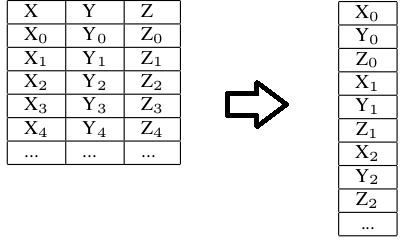
\includegraphics[bb=0 0 400 241,scale=0.5]{refs/ThisBecomesThat.png}
  \end{center}
  \caption{Population Individual Modification}
  \label{fig:postOpExplain}
\end{figure}

\subsection{Fitness}

The goal of the experiment is to find an atomic structure that generates the same EXAFS spectra as the experimental EXAFS spectra. If an atomic structure were to be generated that produces the same EXAFS spectra as the one found in experimentation then it can be said that the real atomic structure would have been found.

To calculate how close the calculated EXAFS spectra is to the experimental EXAFS spectra, root-mean-square deviations (RMSD), see Equation~\ref{eq:rmsdFormula}, will be computed between the calculated and experimental spectra. Each spectra is recorded at increments of 0.05 $k \mathbin{/} A\textsuperscript{-1}$ which allows $EXAFS \chi k\textsuperscript{3}$ to be compared at each increment. The goal is to get the RMSD value as low as possible because then the calculated and experimental EXAFS spectra match as closely as possible. It is not reasonable to expect the RMSD to be zero, because the experimental EXAFS spectra isn't perfect. The environment in which the EXAFS spectra is recorded creates small errors in the result.

\begin{equation}
  \label{eq:rmsdFormula}
  RMSD = \sqrt{\frac{\sum_{t=1}^{n} \left ( x_{1,t}-x_{2,t} \right )^{2}}{n}}
\end{equation}

\subsection{Population}
\label{sec:population}

The initial OEC atomic structure came from the crystallographic photosystem II (PSII) structure~\cite{umena2011crystal}. It is available in the Protein Data Bank (PDB)~\cite{databank} as PDB ID 3ARC. It was used as a starting point for the experiments. To ensure that the atomic structure was as stable as possible, the structure was put into a molecular dynamics simulation and the atoms were allowed to move freely in space until the overall temperature of the system was reasonably low. This acted as the baseline atomic structure for all tests. NAMD~\cite{namd} was used for the molecular dynamics simulations.

In order to generate the initial population, two different approaches were used. At first, the individual atom coordinates were randomly shifted to generate a population but during the EXAFS analysis too many invalid atomic structures were being generated. An invalid atomic structure could be attributed to multiple reasons but the most common reason is that the atoms are overlapping or are too close together. The second approach taken was to let a molecular dynamics simulation generate an initial population. In this approach, the atomic structure was run through the molecular dynamics simulation again but instead the temperature of the system would be increased in order to make the atoms oscillate. The molecular dynamics simulation was allowed to run for 10000 steps. Each of these steps represents a unique atomic structure of the OEC and these were used to seed the genetic algorithm's population.

The atomic structures that were generated contained 1269 chemical elements. For the purposes of OEC structure refinement only 79 specific atoms were required for EXAFS analysis. The genetic algorithm only used the 79 atoms that required refinement. The generated atomic structures were run through IFEFFIT and compared to the target EXAFS spectra. The top 3\% (roughly 300) were used to generate the initial populations in the genetic algorithm.

\subsection{Crossover operator}

Two individuals are selected from the population and one-point crossover is performed. A random integer value is chosen based on the number of atoms in the individual, and the two individuals will trade their atomic positions based on the pivot point. One point crossover was chosen because it is less destructive to the individuals than other forms of crossover.

\subsection{Mutation operator}
\label{subsec:mutation}

For the mutation operator a single atom coordinate will be moved. A random atomic coordinate is selected from the individual and its position is moved randomly by 0.05\AA\  using Euclidean distance. The resulting position will be 0.05\AA\ away from its original position. In order to determine how much distance the atomic position should be moved, an analysis was needed to learn more about how changing atomic positions affects the calculated EXAFS spectra.

The analysis consisted of moving each atom, individually, in a variety of directions and calculating its RMSD score. Each atom was moved in a total of six directions ($\pm$X, $\pm$Y, and $\pm$Z), at a variety of distances (0.001\AA, 0.005\AA, 0.01\AA, 0.025\AA, 0.05\AA, 0.1\AA, 0.5\AA, 1\AA, and 5\AA). This was done to determine how much movement was required of an atom to make a significant change to the RMSD score. Table~\ref{table:minMove} shows results of how much movement is required to produce a 1\% and 5\% change to their RMSD scores. Since there is more than one instance of each chemical element in OEC, the distance chosen was the first distance that produced the minimum change because the goal was to find the absolute minimum for each chemical element.

\begin{table}
\caption{Minimum Move Required at 1\%}
\label{table:minMove}
\centering
\normalsize
\begin{tabular}{ | l | l | l | }
  \hline
    Element & 1\% Difference & 5\% Difference \\ \hline
    O & 0.025\AA & 0.5\AA \\ \hline
    Mn & 0.01\AA & 0.5\AA \\ \hline
    Ca & 1\AA & 5\AA \\ \hline
    C & 0.5\AA & 5\AA \\ \hline
    N & 0.5\AA & 5\AA \\ \hline
    H & 5\AA & 5\AA \\ \hline
\end{tabular}
\end{table}

The value of 0.05\AA\ was chosen for the experiments as a middle ground that could be applied to each chemical element. It should be noted that the value of 0.05\AA\ is particular to OEC. A similar analysis could be done to determine the minimum move distance for each element in another chemical complex.

\subsection{Selection operator}

For the selection operator a 3-tournament selection was used.

\subsection{Restarting}
\label{subsec:restarting}

For the implementation of RGA, each run was seeded with 300 unique individuals. The initial population only used the specific amount of individuals it needed at generation 0 and during each population restart duplicates in the population re replaced with new individuals from the original 300. Figure~\ref{fig:bestRunRestarting} demonstrates how a population looks while restarting is occurring. Restarting has occurred at generations 19, 35, 46, and 71. The periodic decreases in fitness are destructive to the population but overall a consistent improvement in the fitness is seen throughout the run. The new individuals that are injected into the population allow for continued improvement to the fitness.

\begin{figure}
\begin{center}
\begin{tikzpicture}
  \begin{axis}[
    % width=15cm,
    % height=8cm,
    grid=both,
    title={Best RGA Run},
    legend entries={Best,Average},
    xlabel={Generations},
    ylabel={RMSD}
  ]

  \addplot[mark=x] table [col sep=comma,y index=1, x index=0] {results/best_run/results-fixed.csv};
  \addplot[mark=*] table [col sep=comma,y index=2, x index=0] {results/best_run/results-fixed.csv};

  \end{axis}
\end{tikzpicture}
\end{center}
\caption{Example of a Restarting Genetic Algorithm}
\label{fig:bestRunRestarting}
\end{figure}

\subsection{Experiments}

The GA and RGA will be performed as direct comparisons with each other. The variety of system parameters tested can be seen in Table~\ref{table:gaParameters}. A population size of 50 was selected as a result of empirical testing. It was found that using a population size of less than 50 did not provide enough diversity within the population and using a population size of greater than 50 had no impact of the results. The number of runs was decided to be 10 in order to obtain sensible results in a reasonable amount of time.

\begin{table}
\caption{System Parameters used in GA and RGA}
\label{table:gaParameters}
\centering
\begin{tabular}{ | l | r | }
  \hline
    Settings & Values \\ \hline \hline
    Runs & 10 \\ \hline
    Generations & Max. 30, Until Converged \\ \hline
    Population Size & 50 \\ \hline
    Crossover Rate & 80, 70 \\ \hline
    Mutation rate & 10, 20, 30 \\ \hline
    Elitism & True, False \\ \hline
    Number of restart attempts & 3, 5 \\ \hline
    Max convergence percentage before restarting & 5\%, 10\% \\ \hline
\end{tabular}
\end{table}

\subsection{Results and Discussion}

Table~\ref{table:sampleRuns} contains a summary of the GA and RGA experiments. Immediately it is clear that the RGA outperforms the GA. A closer look revealed that the basic GA experiments were converging early on local optima. The RGA experiments initially converged on similar optima but were able to find new optima after each restarting phase. The RGA performed better than the GA but required more than double the amount of generations. Figure~\ref{fig:bestRunRestarting} provides an example of the generational data for the best run of RGA.

The average RMSD score from the RGA was able to outperform both benchmark RMSD scores but only by a small margin. Fortunately, because the goal is to find a single individual, the best candidate solution from the RGA was able to far exceed the benchmark scores with RMSD of 1.0877. Figure~\ref{fig:bestRunEXAFS} shows the comparison of the EXAFS spectra.

After examining the calculated EXAFS spectra and the experimental EXAFS spectra it becomes clear that the calculated EXAFS spectra will never exactly fit the experimental EXAFS spectra. In particular, there appears to be many jagged jumps along the experimental EXAFS spectra that create many difficulties for matching by the calculated EXAFS spectra. Nonetheless, this can produce a good approximation for further experimentation.

\begin{table}
  \caption{Results from GA and RGA Experiments}
  \label{table:sampleRuns}
  \centering
  \begin{tabular}{ | l | l | l | l | l | l | l | l | l | l | }
    \hline
    Gen. & Crossover & Mutation & Elitism & Conv. Rate & Restarting &  Avg. Best \\ \hline \hline
    30 & 80\% & 20\% & False & - & - & 1.3411 \\ \hline
    30 & 80\% & 10\% & False & - & - & 1.3746 \\ \hline
    30 & 70\% & 30\% & False & - & - & 1.2756 \\ \hline
    30 & 80\% & 10\% & True & - & - & 1.3278 \\ \hline
    30 & 70\% & 30\% & True & - & - & 1.2591 \\ \hline
    30 & 80\% & 20\% & True & - & - & 1.3299 \\ \hline
    67 & 80\% & 20\% & True & 10\% & 3 & 1.2247 \\ \hline
    81 & 80\% & 20\% & True & 5\% & 3 & 1.2117 \\ \hline
    107 & 80\% & 20\% & True & 10\% & 5 & 1.2062 \\ \hline
    124 & 80\% & 20\% & True & 5\% & 5 & 1.2156 \\ \hline
    67 & 70\% & 30\% & True & 5\% & 5 & \textbf{1.1998} \\ \hline
    81 & 70\% & 30\% & True & 10\% & 5 & 1.2138 \\ \hline
  \end{tabular}
\end{table}

\begin{figure*}
\begin{center}
\begin{tikzpicture}
  \begin{axis}[
    width=16cm,
    height=6cm,
    grid=both,
    title={EXAFS Spectra in k space},
    legend entries={Experimental,Calculated},
    legend pos=south east,
    xlabel={$k \mathbin{/} A\textsuperscript{-1}$},
    ylabel={$EXAFS \chi k\textsuperscript{3}$}
  ]

  \addplot[mark=x] table [col sep=comma,y index=1, x index=0] {results/best_run/for_chart.csv};
  \addplot[mark=*,mark size=1] table [col sep=comma,y index=2, x index=0] {results/best_run/for_chart.csv};

  \end{axis}
\end{tikzpicture}
\end{center}
\caption{OEC EXAFS Spectra Comparison}
\label{fig:bestRunEXAFS}
\end{figure*}

\subsection{Post-Optimization}

Post-optimization was performed because the search space is too large to search every possible configuration. Algorithms based on continuous space problems were not very successful at developing good solutions to the problem. PSO and DE were originally tested against the RGA performance but the results were not promising. Once the RGA was able to produce high quality solutions for OEC these candidate solutions were applied to PSO and DE as an attempt at post-optimization. 

A candidate solution found from the GA experiments was used to seed the initial population of the PSO and DE algorithms. The peer-reviewed computational intelligence library, CILIB~\cite{cilib}, was used to run the PSO and DE experiments.

To generate the initial population, for both PSO and DE, each floating point value within each individual was randomly adjusted by a range of numbers. At first adjusting each value by $\pm$1\AA\ was tried but the results were far worse than the original candidate solution. Improvements did not begin to appear until the adjusted amount was significantly reduced. Ranges of $\pm$0.05\AA\ and $\pm$0.25\AA\ were used to generate improved results. Table \ref{table:localResults} shows the results of the two post-optimization strategies. These scores are averaged over 30 runs.

\begin{table}
\caption{Local Search Results}
\label{table:localResults}
\centering
\begin{tabular}{ | l | l | l | l | l | }
  \hline
    Algorithm & Initial Movement Radius & Pop. Size & Gen. & Average Best \\ \hline
    PSO & $\pm$0.05\AA & 50 & 100 & 0.7782 \\ \hline
    PSO & $\pm$0.05\AA & 50 & 30 & 0.8976 \\ \hline
    PSO & $\pm$0.25\AA & 50 & 30 & 1.2411 \\ \hline
    DE & $\pm$0.05\AA & 50 & 30 & 1.1354 \\ \hline
    DE & $\pm$0.25\AA & 50 & 30 & 1.7220 \\ \hline
\end{tabular}
\end{table}

The results of the DE experiments were not promising. Results were improving but their RMSD scores never improved past the candidate solutions. In contrast, the results of the PSO experiments were extremely successful. Figure \ref{fig:psoResults} shows the generational results of the PSO averaged over 30 runs. The RMSD score of the candidate solution was significantly reduced which shows that PSO works very well as a post-optimization strategy. 

\begin{figure}[H]
\begin{center}
\begin{tikzpicture}
  \begin{axis}[
    % width=15cm,
    % height=8cm,
    grid=both,
    title={PSO Fitness},
    legend entries={$\pm$0.05, $\pm$0.25},
    xlabel={Generations},
    ylabel={RMSD}
  ]

  \addplot[mark=*] table [col sep=comma,y index=1, x index=0] {results/cilib/pso/0.1/results-fixed.csv};
  \addplot[mark=-] table [col sep=comma,y index=1, x index=0] {results/cilib/pso/0.5/results-fixed.csv};

  \end{axis}
\end{tikzpicture}
\end{center}
\caption{PSO Post-Optimization Results}
\label{fig:psoResults}
\end{figure}

The results from the PSO and DE experiments using different initial movement radii were very surprising. Using a smaller initial movement radius suggests that the initial candidate solution is already very close to the ideal solution. The PSO was able to improve the best candidate by almost 50\%. Figure~\ref{fig:psoBestRunEXAFS} shows the best EXAFS spectra after optimization from the PSO which has an RMSD score of 0.7287.

\begin{figure*}
\begin{center}
\begin{tikzpicture}
  \begin{axis}[
    width=16cm,
    height=6cm,
    grid=both,
    title={EXAFS Spectra in k space},
    legend entries={Experimental,Calculated},
    legend pos=south east,
    xlabel={$k \mathbin{/} A\textsuperscript{-1}$},
    ylabel={$EXAFS \chi k\textsuperscript{3}$}
  ]

  \addplot[mark=x] table [col sep=comma,y index=2, x index=0] {results/pso_results/pso-100.csv};
  \addplot[mark=*,mark size=1] table [col sep=comma,y index=1, x index=0] {results/pso_results/pso-100.csv};

  \end{axis}
\end{tikzpicture}
\end{center}
\caption{OEC EXAFS Spectra Comparison for PSO Post-Optimization}
\label{fig:psoBestRunEXAFS}
\end{figure*}

\section{Subset Testing}
\label{sec:subsetTesting}

In an attempt to reduce the search space of the problem, different chemical elements were left rigid during the evolutionary process. Table \ref{table:elementBreakdown} gives a breakdown of the atoms contained within OEC.

Experiments were run on different subsets of chemical elements. Each subset was allowed to move freely while the chemical elements not listed were kept rigid. Table \ref{table:subsetResults} demonstrates the results over 10 runs. Certain rows in Table \ref{table:subsetResults} contain \textbf{N/A} as their values were too large. The atoms listed in each row were allowed to be flexible during the experiment. The parameters were kept consistent for each experiment and can be seen in Table \ref{table:subsetParameters}.

\begin{table}
\caption{Chemical Element Breakdown}
\label{table:elementBreakdown}
\centering
\normalsize
\begin{tabular}{ | l | l | }
  \hline
    Element & Count \\ \hline
    Mn & 4 \\ \hline
    Ca & 1 \\ \hline
    O & 26 \\ \hline
    C & 14 \\ \hline
    N & 6 \\ \hline
    H & 28 \\ \hline
    Total & 79 \\ \hline
\end{tabular}
\end{table}

\begin{table}
  \caption{Experiments with different subsets}
  \label{table:subsetResults}
  \centering
  \normalsize
  \begin{tabular}{ | l | l | l | }
    \hline
    Atoms & Best & Average \\ \hline \hline
    Mn, Ca, C, O, N, H & 1.1998 & 1.2580 \\ \hline
    Mn, Ca, C, O, N & 1.1697 & 1.2621 \\ \hline
    Mn, Ca, C & 2.4413 & N/A \\ \hline
    Mn, Ca, O & 1.2531 & N/A \\ \hline
    Mn, Ca, N & 2.4881 & N/A \\ \hline
    Mn, Ca, C, O & 1.1648 & N/A \\ \hline
    Mn, Ca, C, N & 2.5143 & 2.5649 \\ \hline
    Mn, Ca, O, N & N/A & N/A \\ \hline
    Mn, Ca & 2.4916 & 2.5088 \\ \hline
  \end{tabular}
\end{table}

\begin{table}
\caption{GA Subset Parameters}
\label{table:subsetParameters}
\centering
\normalsize
\begin{tabular}{ l r }
  \hline
    Runs & 10 \\
    Population size & 50 \\
    Crossover rate & 0.7 \\
    Mutation rate & 0.3 \\
    Elitism & True \\
    Number of restart attempts & 5 \\
    Max convergence percentage before restarting & 5\% \\
  \hline
\end{tabular}
\end{table}

The results of the experiments revealed some interesting characteristics. Having the Hydrogen elements rigid actually produces improved results. This is not surprising since early examination of the atoms revealed that moving a Hydrogen element had very little impact on the RMSD score. It is suspected that the RMSD score has improved because the chromosome length has been reduced from 79 to 51. The reduced chromosome length would allow for more different combinations to be attempted. This idea will be examined in more detail in future work, as discussed in Section~\ref{sec:conclusion}.

\section{Conclusion and Future Work}
\label{sec:conclusion}

This work shows that the GA and RGA were able to produce comparable atomic structures to those of existing solutions. The RGA was able to outperform existing solutions but only by a small margin. Using PSO as a post-optimization technique was able to significantly improve the solutions found by the RGA. Table~\ref{table:resultsComparison} shows a comparison of the best results found using RGA and PSO.

\begin{table}
\caption{Comparison of Results}
\label{table:resultsComparison}
\centering
\normalsize
\begin{tabular}{ | l | l | l | l | l | }
  \hline
    Algorithm & Best Results \\ \hline
    DFT-QM/MM~\cite{luber2011s1} & 1.2643 \\ \hline
    R-QM/MM~\cite{luber2011s1} & 1.2403 \\ \hline
    RGA & 1.0877 \\ \hline
    PSO & 0.7287 \\ \hline
\end{tabular}
\end{table}

In the initial stages of this work PSO and GA were used for testing but the PSO was not able to perform with any reasonable success. With the improvements the PSO was able to make to the RGA results, more testing is required using the PSO. It is possible that the initial poor results from the PSO are due to the initial population. In the future an alternative method of generating a population for PSO and DE should be considered.

The study performed in Section~\ref{subsec:mutation} was done to determine how much an atom should be shifted during the mutation phase. The analysis revealed that different chemical elements require different minimum distances to create a noticeable effect on the RMSD score. In this work the each atom is treated the same way and shifted by the absolute minimum distance found. Future work should attempt to shift each atom by their own minimum distances, thereby allowing for more precise results.

The molecular dynamics simulation performed to create the initial population was useful in creating candidate solutions for the GA. Using the molecular dynamics simulation should be studied as a way of restarting the GA. Once the best candidate solution is found using the GA it should be placed back in the molecular dynamics simulation to generate new atomic structures that could be used to restart the GA.

It should be noted that the results in this work have not been tested for chemical feasibility. In particular, subset testing was performed as a proof of concept for future work. The exploration of subset testing in this work may be producing results that are chemically infeasible. To solve this problem, the created atomic structure should be placed in the molecular dynamics program,  discussed in Section~\ref{sec:population}, to optimize the positions of the rigid chemical elements.

A secondary goal, that is not explored in this work, of atomic structure refinement is to generate atomic structures that produce a low potential energy. Some configurations of the atomic structure produce chemically unreasonable structures meaning that their potential energy is too high or they cannot exist in nature. The atomic structures should be analyzed using force fields to measure their feasibility and potential energy.

A benefit of using a population based algorithm is that at the end of a run there are several possible candidate solutions. For the purposes of atomic structure refinement using EXAFS Spectra analysis having a set of candidate solutions is actually beneficial because each candidate solution is going to have different chemical properties. Further analysis of these individuals, by an expert, could expose which candidates are most suitable.

A multi-objective approach could be applied to molecular structure refinement since the ideal model would have both a low RMSD score and low potential energy. The cost of adding the force field calculations would double the time required to evaluate an individuals fitness, which is already significantly high. A possible solution to incorporating force field calculations without significantly increasing the evalution time would be to only calculate the individual's potential energy on a generational interval but this still demands research.

% \subsection{GA Parameters}

% \begin{table}[H]
% \caption{GA Parameters}
% \centering
% \begin{tabular}{ l r }
%   \hline
%     Population size & 50 \\
%     Crossover rate & 0.8 \\
%     Mutation rate & 0.2 \\
%     Elitism & True \\
%     Number of restart attempts & 5 \\
%     Max convergence percentage before restarting & 5\% \\
%   \hline
% \end{tabular}
% \end{table}

% \begin{table}[htp]
% \caption{Sample Chromosome Representation}
% \label{tab:sampleChromosome}
% \centering
% \begin{tabular}{ | l | l | l |}
%   \hline
%     X & Y & Z \\ \hline
%     X$_0$ & Y$_0$ & Z$_0$ \\ \hline
%     X$_1$ & Y$_1$ & Z$_1$ \\ \hline
%     X$_2$ & Y$_2$ & Z$_2$ \\ \hline
%     X$_3$ & Y$_3$ & Z$_3$ \\ \hline
%     X$_4$ & Y$_4$ & Z$_4$ \\ \hline
%     ... & ... & ... \\ \hline
% \end{tabular}
% \end{table}

% \begin{table}[htp]
% \caption{Sample Chromosome Representation}
% \label{tab:sampleChromosome2}
% \centering
% \begin{tabular}{ | c |}
%   \hline
%     X$_0$ \\ \hline
%     Y$_0$ \\ \hline
%     Z$_0$ \\ \hline
%     X$_1$ \\ \hline
%     Y$_1$ \\ \hline
%     Z$_1$ \\ \hline
%     X$_2$ \\ \hline
%     Y$_2$ \\ \hline
%     Z$_2$ \\ \hline
%     ... \\ \hline
% \end{tabular}
% \end{table}

% An example of a floating figure using the graphicx package.
% Note that \label must occur AFTER (or within) \caption.
% For figures, \caption should occur after the \includegraphics.
% Note that IEEEtran v1.7 and later has special internal code that
% is designed to preserve the operation of \label within \caption
% even when the captionsoff option is in effect. However, because
% of issues like this, it may be the safest practice to put all your
% \label just after \caption rather than within \caption{}.
%
% Reminder: the "draftcls" or "draftclsnofoot", not "draft", class
% option should be used if it is desired that the figures are to be
% displayed while in draft mode.
%
%\begin{figure}[!t]
%\centering
%\includegraphics[width=2.5in]{myfigure}
% where an .eps filename suffix will be assumed under latex, 
% and a .pdf suffix will be assumed for pdflatex; or what has been declared
% via \DeclareGraphicsExtensions.
%\caption{Simulation Results}
%\label{fig_sim}
%\end{figure}

% Note that IEEE typically puts floats only at the top, even when this
% results in a large percentage of a column being occupied by floats.


% An example of a double column floating figure using two subfigures.
% (The subfig.sty package must be loaded for this to work.)
% The subfigure \label commands are set within each subfloat command, the
% \label for the overall figure must come after \caption.
% \hfil must be used as a separator to get equal spacing.
% The subfigure.sty package works much the same way, except \subfigure is
% used instead of \subfloat.
%
%\begin{figure*}[!t]
%\centerline{\subfloat[Case I]\includegraphics[width=2.5in]{subfigcase1}%
%\label{fig_first_case}}
%\hfil
%\subfloat[Case II]{\includegraphics[width=2.5in]{subfigcase2}%
%\label{fig_second_case}}}
%\caption{Simulation results}
%\label{fig_sim}
%\end{figure*}
%
% Note that often IEEE papers with subfigures do not employ subfigure
% captions (using the optional argument to \subfloat), but instead will
% reference/describe all of them (a), (b), etc., within the main caption.


% An example of a floating table. Note that, for IEEE style tables, the 
% \caption command should come BEFORE the table. Table text will default to
% \footnotesize as IEEE normally uses this smaller font for tables.
% The \label must come after \caption as always.
%
%\begin{table}[!t]
%% increase table row spacing, adjust to taste
%\renewcommand{\arraystretch}{1.3}
% if using array.sty, it might be a good idea to tweak the value of
% \extrarowheight as needed to properly center the text within the cells
%\caption{An Example of a Table}
%\label{table_example}
%\centering
%% Some packages, such as MDW tools, offer better commands for making tables
%% than the plain LaTeX2e tabular which is used here.
%\begin{tabular}{|c||c|}
%\hline
%One & Two\\
%\hline
%Three & Four\\
%\hline
%\end{tabular}
%\end{table}


% Note that IEEE does not put floats in the very first column - or typically
% anywhere on the first page for that matter. Also, in-text middle ("here")
% positioning is not used. Most IEEE journals/conferences use top floats
% exclusively. Note that, LaTeX2e, unlike IEEE journals/conferences, places
% footnotes above bottom floats. This can be corrected via the \fnbelowfloat
% command of the stfloats package.






% conference papers do not normally have an appendix


% use section* for acknowledgement
\section*{Acknowledgment}

This research was supported in part by the Natural Sciences and Engineering Research Council of Canada.

The authors would like to thank Christian Negre for providing EXAFS Spectra data for OEC S$_{1}$ and James Hughes for helpful comments on preparing this work.

% trigger a \newpage just before the given reference
% number - used to balance the columns on the last page
% adjust value as needed - may need to be readjusted if
% the document is modified later
%\IEEEtriggeratref{8}
% The "triggered" command can be changed if desired:
%\IEEEtriggercmd{\enlargethispage{-5in}}

% references section

% can use a bibliography generated by BibTeX as a .bbl file
% BibTeX documentation can be easily obtained at:
% http://www.ctan.org/tex-archive/biblio/bibtex/contrib/doc/
% The IEEEtran BibTeX style support page is at:
% http://www.michaelshell.org/tex/ieeetran/bibtex/
\bibliographystyle{IEEEtran}
% argument is your BibTeX string definitions and bibliography database(s)
\bibliography{mybib}
%
% <OR> manually copy in the resultant .bbl file
% set second argument of \begin to the number of references
% (used to reserve space for the reference number labels box)
% \begin{thebibliography}{1}

% \bibitem{IEEEhowto:kopka}
% H.~Kopka and P.~W. Daly, \emph{A Guide to \LaTeX}, 3rd~ed.\hskip 1em plus
%   0.5em minus 0.4em\relax Harlow, England: Addison-Wesley, 1999.

% \bibitem{victor}
% Sandra Luber, Ivan Rivalta, Yasufumi Umena, Keisuke Kawakami, Jian-Ren Shen, Nobuo Kamiya, Gary W. Brudvig, and Victor S. Batista, \emph{S$_{1}$-State Model of the O$_{2}$-Evolving Complex of Photosystem II.} 2011 American Chemical Society

% \bibitem{victor2}
% Eduardo M. Sproviero , José A. Gascón †, James P. McEvoy ‡, Gary W. Brudvig and Victor S. Batista, \emph{A Model of the Oxygen-Evolving Center of Photosystem II Predicted by Structural Refinement Based on EXAFS Simulations.}

% \bibitem{a}
% G. Charles Dismukes, and Rogier T. van Willigen, \lq\lq Manganese: The Oxygen-evolving Comlpex & Models,\rq\rq 


% \end{thebibliography}




% that's all folks
\end{document}


